\chapter{Results and summary}
  In the previous two chapters the analysis steps to measure the coherent
    \JPsi{} photoproduction were given.
  In this chapter, the measured cross section for this process is given
    in Section~\ref{sec:jpCoRes}.
  Comparisons to the theoretical models are discussed. 
  In addition, the rapidity correlation between UPC \JPsi{} and forward
    neutrons are presented and compared to model calculations in 
    Section~\ref{sec:upcCor}. 
  Finally, a summary of the complete thesis is given.  
  
  \section{Coherent \JPsi{} cross section\label{sec:jpCoRes}}
  %
    The coherent \JPsi{} cross section is calculated using the following
      formula:
  %
    \begin{equation}
    \frac{d\sigma^{J/\psi}_{coh}}{dy} (Xn0n)= \frac{N^{J/\psi}_{coh}}{\mathcal{L} \cdot (2 \cdot \Delta y )\cdot BR}~\textrm{,}
    \label{eq:expXSecCo}
    \end{equation}
  %
      where $N^{J/\psi}_{coh}$ is the corrected number of coherent $J/\psi$
      candidates,  $\mathcal{L}$ is the integrated luminosity used for this 
      analysis, $\Delta y$ is the width of the rapidity interval, and $BR$ is 
      the branching ratio for \JPsi{} to $\mu^{+}\mu^{-}$. 
    To obtain $N^{J/\psi}_{coh}$ the following formula was used:
  %
    \begin{equation}
    N^{J/\psi}_{coh}(Xn0n) = \frac{N^{J/\psi}_{yield}}{(A\times \varepsilon) \cdot \varepsilon^{ZDC}_{trig} \cdot \varepsilon^{J/\psi}_{trig}}~\textrm{,}
    \end{equation}
  %
      where $N^{J/\psi}_{yield}$ is the $J/\psi$ yield with a $p_{T} <$ 0.15 
      GeV, $A\times \varepsilon$ is the combined acceptance and efficiency, 
      $\varepsilon^{ZDC}_{trig}$ is the ZDC triggering efficiency for detecting
      at least one neutron emitted in the forward region, and 
      $\varepsilon^{J/\psi}_{trig}$ is the $J/\psi$ trigger efficiency measured
      by the ``tag and probe'' method. 
    Each of these quantities can be found in Table~\ref{tab:nJpCoh}.
  %
    \begin{table}
      \centering
      \begin{tabular}{|c|c|c|c|c|} \hhline{--~--} 
        $N^{J/\psi}_{yield}$ & 65 $\pm$ 12 & & $N^{J/\psi}_{coh}$  & 1213 $\pm$ 240 \\ \hhline{--~--}  
        $A\times \varepsilon$ & 0.07 & & $\mathcal{L}$ & 143 \\ \hhline{--~--}
        $\varepsilon^{ZDC}_{trig}$ & 0.96 & & $BR$ & 0.0593 \\ \hhline{--~--}
        $\varepsilon^{J/\psi}_{trig}$ & 0.79 $\pm$ 0.05 & & $\Delta y$ & 0.2 \\ \hhline{--~--} \hhline{--~--}
        $N^{J/\psi{}}_{coh} (Xn0n)$ & 1213 $\pm$ 240 & & $\frac{d\sigma^{J/\psi}_{coh}}{dy} (Xn0n)$ & 356 $\pm$ 71 (stat) $^{+43}_{-50}$ (syst) $\mu$b \\  \hhline{--~--}
      \end{tabular}
      \caption{\label{tab:nJpCoh}The measured quantities used to calculate the 
        corrected number of coherent \JPsi{}, $N^{J/\psi}_{coh} (Xn0n)$ (right),
        and the quantities used to calculate the cross section for UPC \JPsi{} 
        photoproduction, $\frac{d\sigma^{J/\psi}_{coh}}{dy} (Xn0n)$ (left).}
    \end{table}  
    
    The coherent J/$\psi$ cross section 
      $\frac{d\sigma^{J/\psi}_{coh}}{dy} (Xn0n)$ requires single-sided neutron
      emission, Xn0n. 
    Previous measurements carried by the ALICE Collaboration measured the cross
      section without any break-up requirement. 
    In order to compare to their results, the cross section is scaled by the 
      factor 5.06 to account for the increase in cross section. 
    This value was obtained from STARlight. 
    The resulting cross section is 1.80 $\pm$ 0.37(stat) $^{+0.22}_{-0.25}$ (syst) mb.
 
    \begin{figure}[!Hhbt]
      \centering
      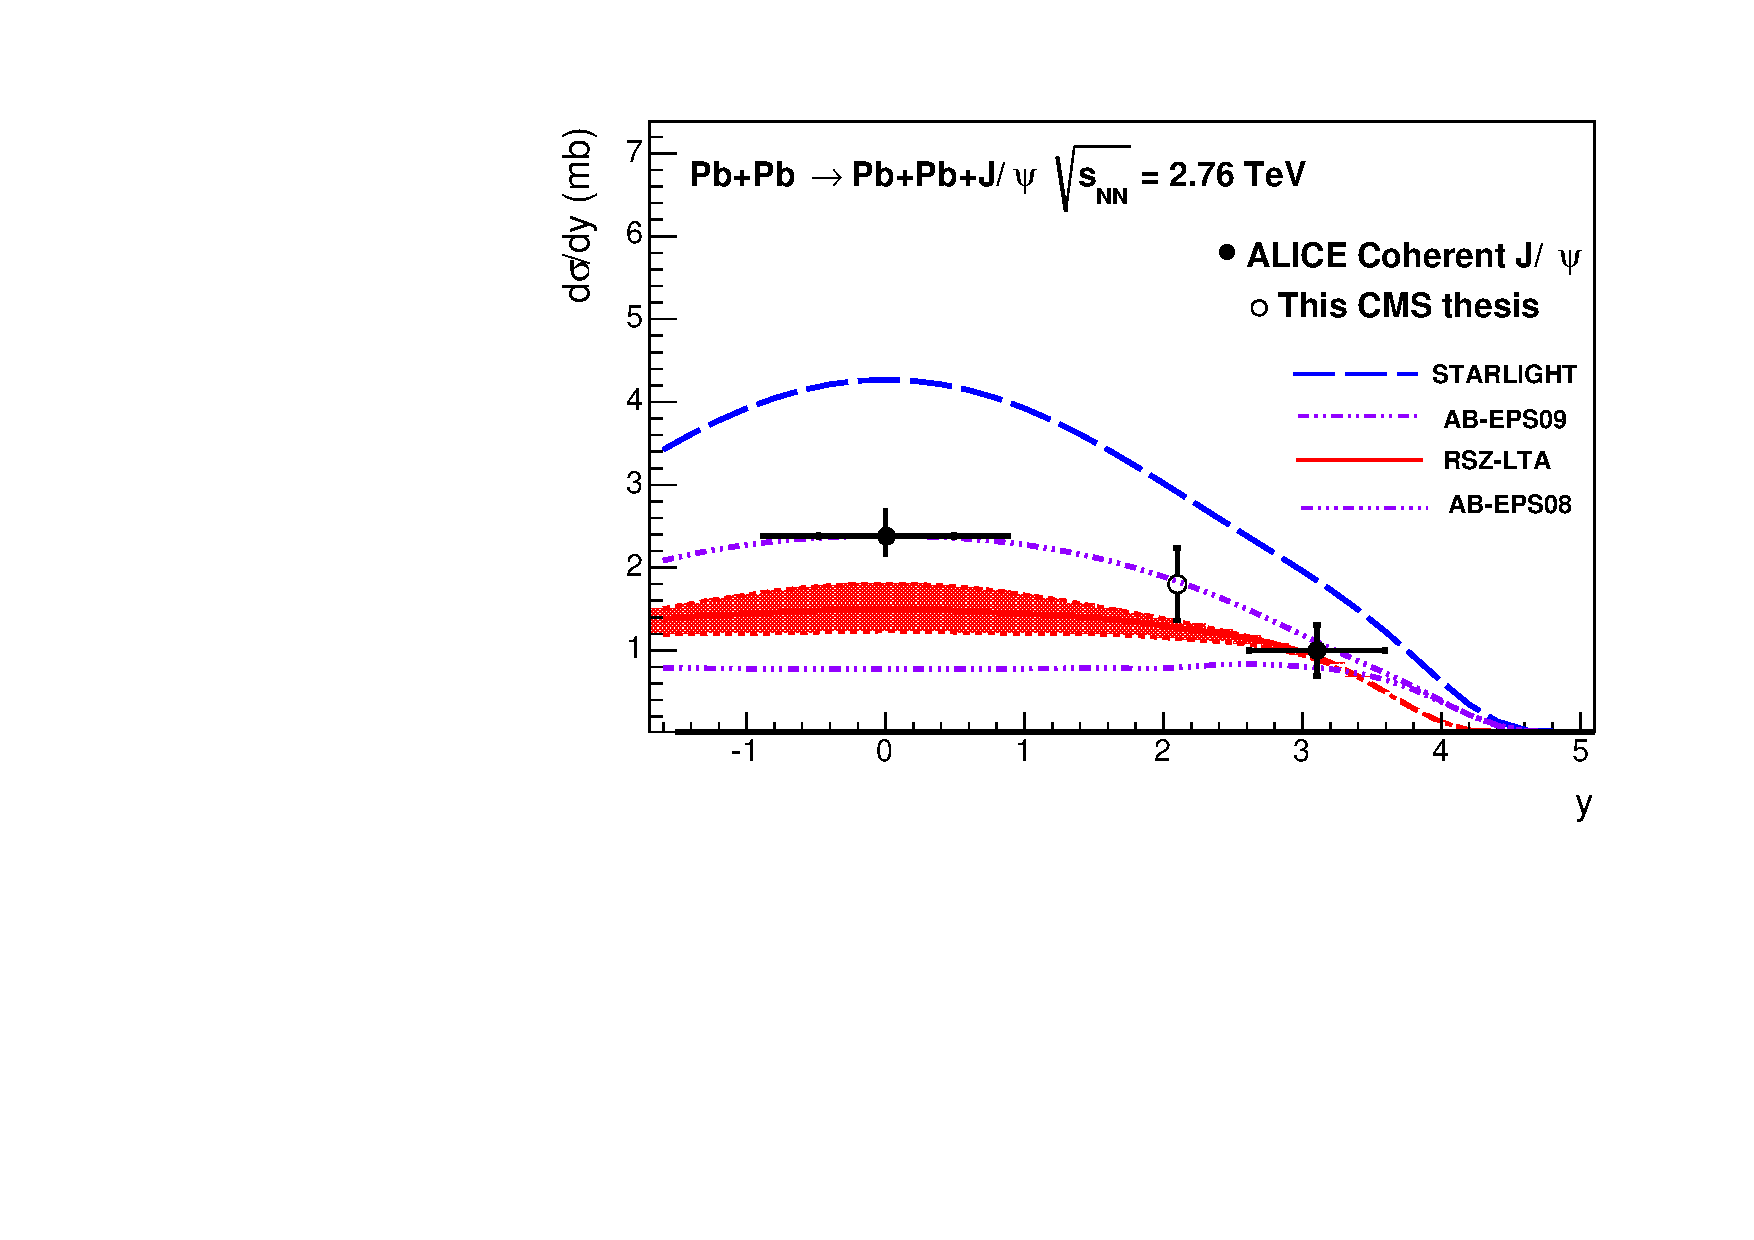
\includegraphics[width=.8\textwidth]{patkenny_thesis}
      \caption{Coherent \JPsi{} photoproduction cross section measured by ALICE 
        and CMS including feed-down and rescaled for nuclear break-up.}
      \label{fig:coJpXsec}
    \end{figure}
    Figure~\ref{fig:coJpXsec} shows the measured cross section compared to the 
      ALICE data points, as well as STARligh, AB and LTA models 
      (see Chapter~\ref{ch:photoNuc}). 
    The measured cross section is in agreement with previous measurements, and 
      favors the AB-EPS09 model. 
    Given the measured cross section is significantly below STARlight, nuclear 
      gluon shadowing plays an important role for $x\sim$ 10$^{-2}$. 

  \section{UPC \JPsi{}-neutron rapidity correlation~\label{sec:upcCor}}
    In addition to the production cross section, neutron dependent
      \JPsi{} photoproduction can be studied in order to better 
      understand the separation between coherent and incoherent photoprodution. 
    Because of the inclusion of the ZDC in the trigger, the data for this 
      thesis is well suited for studying the correlations between the 
      \JPsi{} and neutron rapidities. 
    The difference between neutron emission in coherent and incoherent 
      production was studied in the past \cite{Strikman:2005ze}, and recent
      studies have explored what is possible within the acceptance
      of CMS \cite{Guzey:2013jaa}. 
    In this section, the ratio between \JPsi{}s produced with neutrons in the 
      same side of the detector and opposite side of the detector will be shown
      and compared with theory. 

    Figure~\ref{fig:rNeutDimuCorr} shows the rapidity distribution of UPC 
      \JPsi{} that are accompanied by neutron detection on only one side of the
      interaction point. 
    The candidates are divided by \pt{} and the side of the interaction point
      the neutron was detected in. 
    Low-\pt{} corresponds to the \pt{} < 0.15 GeV, and high \pt{} corresponds
      to 0.15 GeV < \pt < 1 GeV.
    The filled black circles correspond to candidates that are produced in 
      conjunction with a neutron in ZDC$^{-}$, whereas the open squares 
      indicate a neutron in ZDC$^{+}$.
    \begin{figure*}[!Hhtb]
      \begin{center}
        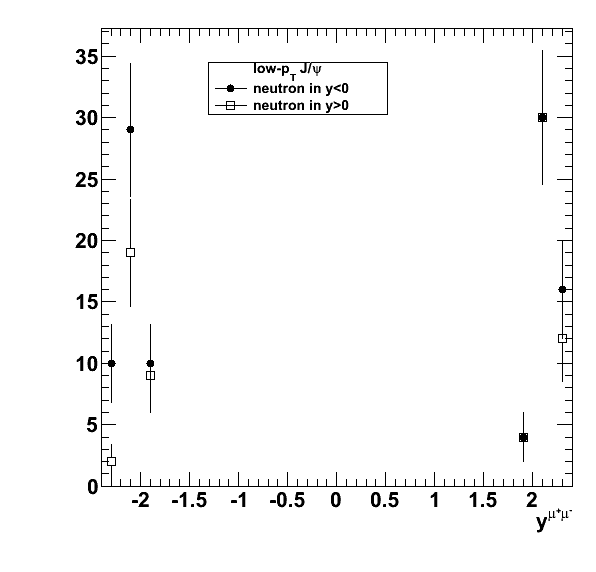
\includegraphics[angle=0,width=0.42\textwidth]{ZDCDimuCorrCoh}
        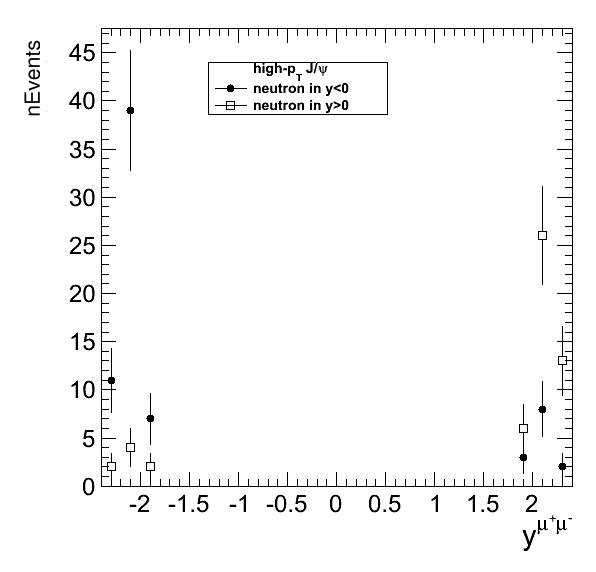
\includegraphics[angle=0,width=0.42\textwidth]{ZDCDimuCorrIncoh}
        \caption{\label{fig:rNeutDimuCorr}Rapidity distribution of \JPsi{} in the
          case of the events having the neutron in negative and positive rapidity 
          for the low-\pt{} \JPsi{} (left), high-\pt{} \JPsi{} (right) and dimuons from
          $\gamma \gamma$ sample (bottom). }
      \end{center}
    \end{figure*}
    In Fig.~\ref{fig:rNeutDimuCorr}, there is a clear preference for the 
      neutron and \JPsi{} to be detected in the same side of the detector for
      the high-\pt{} candidates, however the low-\pt{} candidates do not show
      a strong preference. 

    The ratio between candidates with neutrons on the opposite side of the 
      detector and candidates with neutrons on the same side of the detector,
      $R_{opp/same}$, is measured.
    $R_{opp/same}$ is shown as a function of the candidate \pt{} and compared
      with theory from \cite{Guzey:2013jaa} in Figure~\ref{fig:r2}.
    \begin{figure*}[!Hhtb]
      \begin{center}
        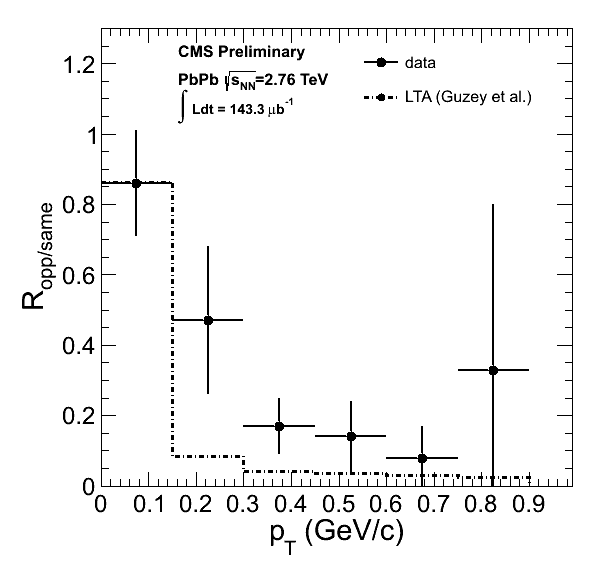
\includegraphics[angle=0,width=0.65\textwidth]{RoppsameVsTheory}
        \caption{\label{fig:r2}Ratio between the transverse momentum 
          distribution of the $J/\psi$ when  $J/\psi$ and neutron have 
          the opposite direction and the transverse momentum distribution 
          of the $J/\psi$ when  $J/\psi$ and neutron have the same direction.}
      \end{center}
    \end{figure*}
    As the \pt{} of the candidates increases beyond 0.3 GeV in Fig.~\ref{fig:r2},
      a transition from \JPsi{} that are uncorrelated with neutron production 
      to \JPsi{} candidates with tend to be created in the same direction as
      the detected neutron. 

    The transition shown in Fig.~\ref{fig:r2} can be explained by the different
      neutron production processes that occur in coherent versus incoherent 
      photoproduction \cite{Strikman:2005ze}.
    In coherent photoproduction, the photon couples elastically to the nucleus 
      as a whole.
    In this case the nucleus will typically stay intact.
    Neutron emission then occurs though exchange of an additional photon. 
    The target struck by this additional photon need not be the same nucleus
      that was the target of the photoproduction process. 
    For this reason, the neutron and \JPsi{} in coherent production are not 
      expected to be correlated.
    Neutron emission in incoherent production is due to the excitation of the 
      nucleus that occurs when the photon couples to an individual nucleon within 
      the nucleus.
    The excited nucleus then decays by neutron emission. 
    In this case, the target nucleus for both the \JPsi{} and the neutron 
       are the same, and there for correlated. 

    The correlation demonstrated in Fig.~\ref{fig:r2} can potentially offer a 
      means of separating the two terms of Eq.\ref{eq:ltaRapDist}, which probe 
      different values of $x$. 
    In incoherent events, because the neutron indicates the direction in which
      the target was traveling, the momentum of the photon can be deduced. 
    If the photon carries higher longitudinal momentum than the gluons with 
      which it interacts, the photoproduced \JPsi{} will be pushed by the 
      photon in the direction opposite the emitted neutron. 
    This would correspond to the low-$x$ contribution to Eq.\ref{eq:ltaRapDist}.
    When the gluons within the nucleus are of higher longitudinal momentum, 
      the \JPsi{} will travel in the direction of the target and the emitted 
      neutron. 
    This gives the high-$x$ contribution. 
    
    The measurement of $R_{opp/same}$ shown in Fig.~\ref{fig:r2} agrees 
      qualitatively with the predictions of \cite{Guzey:2013jaa}.
    This indicates that neutron tagging can both aid in separating the coherent
      from the incoherent process, and potentially separate the low-$x$ and 
      high-$x$ contribution to UPC photoproduction cross sections at high 
      rapidity values. 
    However, this qualitative agreement requires additional theoretical and 
      experimental work for quantitative confirmation. 

  \section{\label{sec:summary}Summary}
    As physicists' understanding of the QGP has deepened over the past 30 years
      of doing experimental heavy ion physics, the questions surrounding the
      QGP have shift from the confirmation of creation of a deconfined state
      to understanding the properties of the state that is created.
    It appears that the QGP is a hot nearly viscosity free fluid of strongly 
      coupled quarks and gluons. 
    The control measurements from dAu collisions at RHIC, and pPb collisions
      at the LHC have shown signs of collective behavior such as flow, which 
      made these results difficult to interpret.
    Additional knowledge of the initial state of the colliding nuclei is needed
      in order to fully understand the QGP signal seen in PbPb and AuAu 
      collisions.
    UPC events can provide this needed knowledge. 
    This thesis contributes to the understanding of the initial state through
      the measurement of the UPC \JPsi{} photoproduction cross section. 
  
    Ultra-peripheral collisions are clean probe of the initial state. 
    In UPC \JPsi{} photoproduction, the nuclei interact through the 
      electromagnetic force precluding the possibility of creating a collective
      medium.
    The theoretical models of coherent UPC \JPsi{} photoproduction model these 
      electromagnetic interactions by combining a semi-classical calculation 
      of the photon flux with a variety of phenomenological and QCD based 
      calculations of the nuclear gluon density. 
    The Weis\"{a}cker-Williams approximation \cite{WWFermi} is used to calculate 
      the flux of photons that surround the colliding nuclei. 
    The interaction of these photons with the nucleus is either calculated 
      through a nuclear modification of the proton gluon density 
      \cite{pQCD2013.02, lta2012.03}, or by using the Glauber model approach 
      that consists in modeling the nucleus as a collection
      of nucleons and scaling the nucleon photoproduction cross sections from 
      e-p collisions \cite{vmd1999}. 
    Photoproduction cross sections from from UPC events can determine at what 
      energy scale the Glauber based method breaks down.
    For the gluon density based calculations, there is a wide discrepancy
      between the predictions, and photoproduction cross sections constrain which
      gluon density models are viable. 
  
    The analysis in this thesis consists of three major components, development
      of a trigger, estimation of efficiency, and measurement of signal events.
    The trigger development involved designing a trigger based on rate estimates
      from past data that ensured a sample that could be used for both measuring
      the signal and estimate the efficiency of the trigger, reconstruction, and
      event selection.
    The number of \JPsi{} candidates was measured by first applying a set 
      of event selection cuts that rejected background events such as hadronic
      collisions and beam gas collisions, then fitting the remaining events to
      templates from simulation to separate the three remaining physics processes,
      the coherent, incoherent, and photon-photon process.
    The efficiencies for each part of the trigger were measured from data. 
    The acceptance and reconstruction efficiency were estimated from MC.
    The cross section was calculated by combining the efficiency with the 
      measured luminosity and number of coherent \JPsi{}.
    The statistical uncertainties were taken from the template fit.
    The systematic uncertainties were estimated by varying the method used on 
      each component of the analysis. 
  
    The UPC \JPsi{} photoproduction cross section in the Xn0n break-up mode, $\frac{d\sigma^{J/\psi}_{co}}{dy}$ (Xn0n),
      was found to be 356 $\pm$ 71 (stat) $^{+43}_{-50}$ (syst) $\mu$b. 
    When rescaled by a factor of 5.06 to account for the difference of break-up mode between 
      the measurement in this thesis and the ALICE result in~\cite{Abelev:2012ba,Abbas:2013oua}, the 
      result of 1.80 $\pm$ 0.37 (stat) $^{+0.22}_{-0.25}$ (syst) mb was found to be consistent with the 
      predictions in \cite{pQCD2013.02}.  
    The calculation in \cite{pQCD2013.02} is also favored by the ALICE measurements. 
    Of the gluon distributions used in \cite{pQCD2013.02}, a gluon distribution with 
      moderately strong gluon shadowing, EPS09~\cite{Eskola:2009uj}, is consistent with both the results from this
      thesis and the previous ALICE results. 
    This indicates that at the scale of the mass of the \JPsi{} the nucleus gluon density is 
      significantly suppressed compared to the gluon densities of a nucleon.
    At this scale the nucleus can not be represented as a collection of nucleons as in the 
      Glauber like model described in \cite{vmd1999}.
    In addition, the \JPsi{}-neutron rapidity correlation shown in Fig.~\ref{fig:r2} by 
      by the $R_{opp/same}$ ratio demonstrates the potential to separate the low-$x$ 
      and high-$x$ contributions to the photoproduction cross section.
  
    The measurements in this thesis confirm the ability to increase the 
      knowledge of the initial state through the exploration of UPC events. 
    This confirmation opens the door to additional measurements in this growing 
      field of UPC research.
    A whole host of measurements will be possible with the data already 
      recorded and with the data that will be recorded in the coming years by 
      CMS and the other LHC experiments.
    UPC photoproduction measurements probing the initial state of the nucleus 
      will play a crucial role in the heavy-ion community as plans for building
      a new electron-ion collider come into focus. 

\iffalse
    In this section the correlation between the rapidity of the $\mu^{+}\mu^{-}$ 
      and of the neutron is studied. The following samples are studied: 
    \begin{itemize}
      \item $\gamma + A$ collisions in which two cases are considered
      \begin{itemize}
        \item elastic coherent interaction: here photon interacts with entire
          nucleus coherently and produce \JPsi. 
          Another photon is needed to cause the breakup and neutron emission. 
          Those two photons are uncorrelated and thus we don't expect to 
            observe the correlation between the rapidity of the neutron and the
            rapidity of the \JPsi.
          In the data sample this corresponds to the low-\pt \JPsi 
            (\pt$<$0.15~GeV). 
        \item inelastic incoherent interaction: here a single high \pt photons
          interacting with nucleus produce the \JPsi and neutron. 
          The correlation between the rapidity of the neutron and the rapidity
            of the \JPsi is expected.
          In the data sample this corresponds to the high-\pt \JPsi 
            (0.15$<$\pt$<$1.05). 
      \end{itemize}
    \end{itemize}

    In order to study the correlation in rapidity between the neutron and
      dimuon direction, four quantities are defined and given in 
      Table~\ref{tab:corrneutronjpsi}.  
    \begin{itemize}
      \item $y^{-}_{\mu\mu} \wedge y_{n}^{-}$: number of $\mu^{+}\mu^{-}$ having
         $y<0$ and the neutron in ZDC$^{-}$ ($y<0$)
      \item $y^{-}_{\mu\mu} \wedge y_{n}^{+}$: number of $\mu^{+}\mu^{-}$ having
         $y<0$ and the neutron in ZDC$^{+}$ ($y>0$)
      \item $y^{+}_{\mu\mu} \wedge y_{n}^{+}$: number of $\mu^{+}\mu^{-}$ having
         $y>0$ and the neutron in ZDC$^{+}$ ($y>0$)
      \item $y^{+}_{\mu\mu} \wedge y_{n}^{-}$: number of $\mu^{+}\mu^{-}$ having
         $y>0$ and the neutron in ZDC$^{-}$ ($y<0$)
    \end{itemize}

    The ratio $R_{opp/same}$ is defined as: 
    \begin{equation}
      R_{opp/same} = \frac{y^{-}_{\mu\mu} \wedge y_{n}^{+} + y^{+}_{\mu\mu} 
        \wedge y_{n}^{-}}{y^{-}_{\mu\mu} \wedge y_{n}^{-} + y^{+}_{\mu\mu} 
        \wedge y_{n}^{+}}.
    \end{equation}
    
    It is seen that the difference between corrected and uncorrected results is
      very small. 
    Other uncertainties cancel. 
    In this case cuts related to the acceptance and efficiencies corrections 
      are not necessary and thus they are released.
    
    Figure~\ref{fig:PtcorrandRation} gives \pt distributions of the \JPsi 
      when the \JPsi{} candidate and neutron have the opposite rapidity 
      direction or when they have the same rapidity direction for low-\pt and 
      high-\pt \JPsi{}. 
    Also the Fig~\ref{fig:PtcorrandRation} gives the $R_{opp/same}$ for low-\pt
      and high-\pt \JPsi. 
    In is send from this plot that in the case of the low-\pt \JPsi this 
      $R_{opp/same}$ ratio is close to 1 and is decreasing when the \pt of
      \JPsi{} increases.
      
    Compiled for \pt$<$1.05~GeV, $R_{opp/same}$ ratio between the \pt 
      distribution of the \JPsi having neutron emitted in the opposite 
      direction and  the \JPsi having the neutron emitted in the same
      direction is shown on Fig.~\ref{fig:r2}. 
    Integrated over rapidity, separately for $y<0$ and $y>0$ ratios from 
      Table~\ref{tab:corrneutronjpsieffcorr} are shown in the 
    
    \begin{figure*}[!Hhtb]
      \begin{center}
        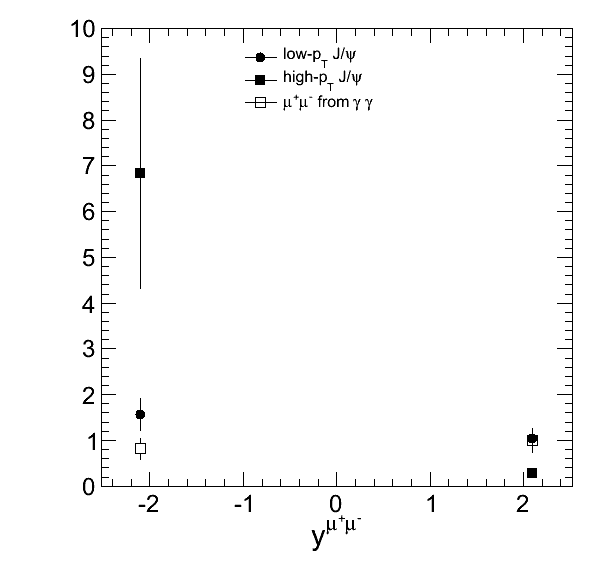
\includegraphics[angle=0,width=0.52\textwidth]{RCompiledYCorr}
        \caption{ \label{fig:integRatios} 
          $R_{(\mu\mu)^{-}}^{\varepsilon_{ZDC}(n^{-}/n^{+})}$ and 
          $R_{(\mu\mu)^{+}}^{\varepsilon_{ZDC}(n^{-}/n^{+})}$ integrated over 
          one side in rapidity for low- and high-\pt \JPsi and also for dimuons
          from $\gamma \gamma$ sample. }
      \end{center}
    \end{figure*}
    From the Tab~\ref{tab:corrneutronjpsi} and the Fig.~\ref{fig:rNeutDimuCorr} 
      it is seen as expected that there is no correlation between the \JPsi 
      rapidity and neutron rapidity in the case of the low-\pt \JPsi and 
      dimuons coming from $\gamma \gamma$ sample. 
    In the case of the high-\pt \JPsi the correlation is clearly visible. 

  \section{Incoherent cross section}
  The same basic procedure for measuring the coherent cross section was used to 
    calculate the incoherent cross section.  
  \section{Break up ratios}
    In Table~\ref{tab:r2} the ratio between raw yields for different break up 
      modes are shown.
    \begin{figure}[!Hhtb]
      \centering
      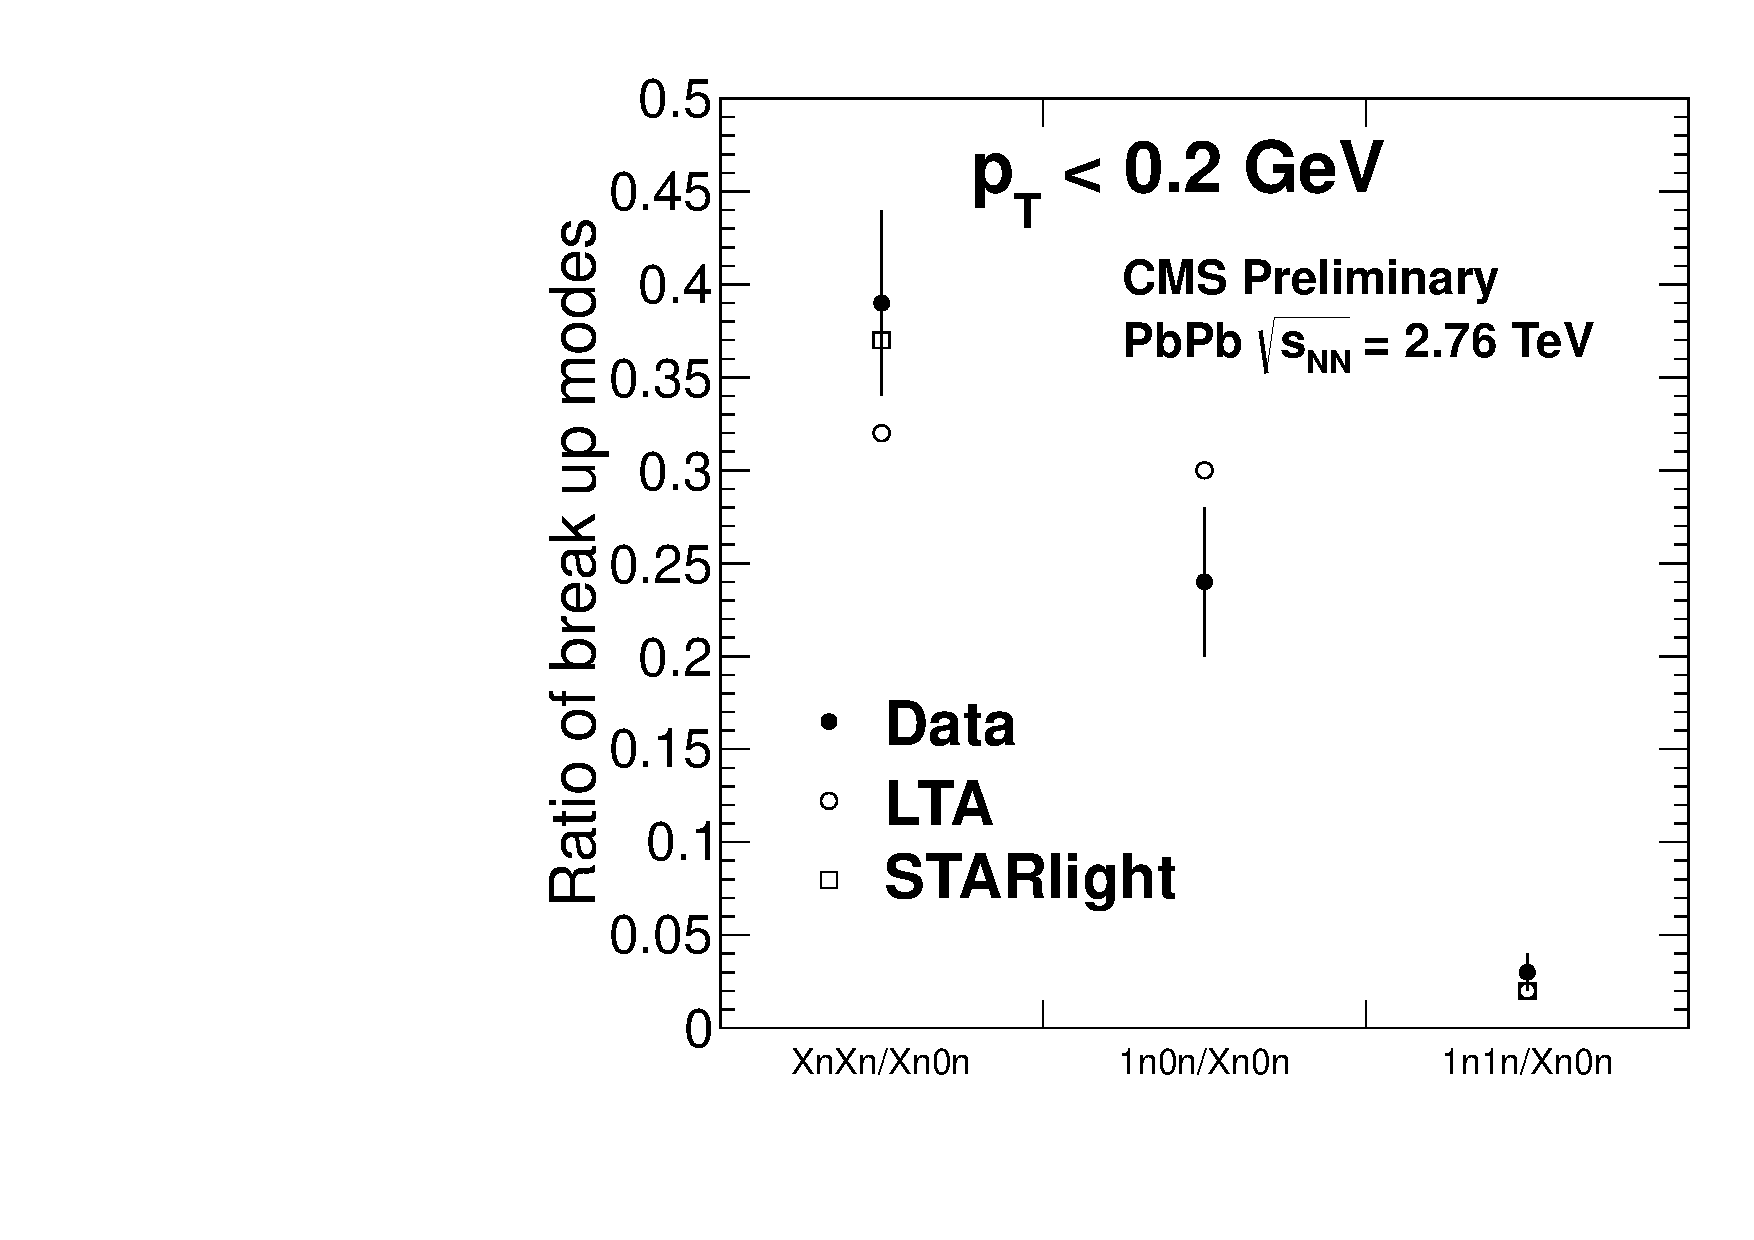
\includegraphics[width=.6\textwidth]{coherentBreakup}
      \caption{Ratio between J/$\psi$ yeilds XnXn and 1n0n break-up modes 
        compared the Xn0n break-up mode for J/$\psi$ with $p_{T}$ below 150 
        MeV.}
      \label{fig:coherentBreakUp}
    \end{figure}
   
    Fig.~\ref{fig:coherentBreakUp} and Fig.~\ref{fig:incoherentBreakUp} compare
      the raw break up ratios two STARlight and LTA predictions. 
    \begin{figure}[!Hhtb]
      \centering
      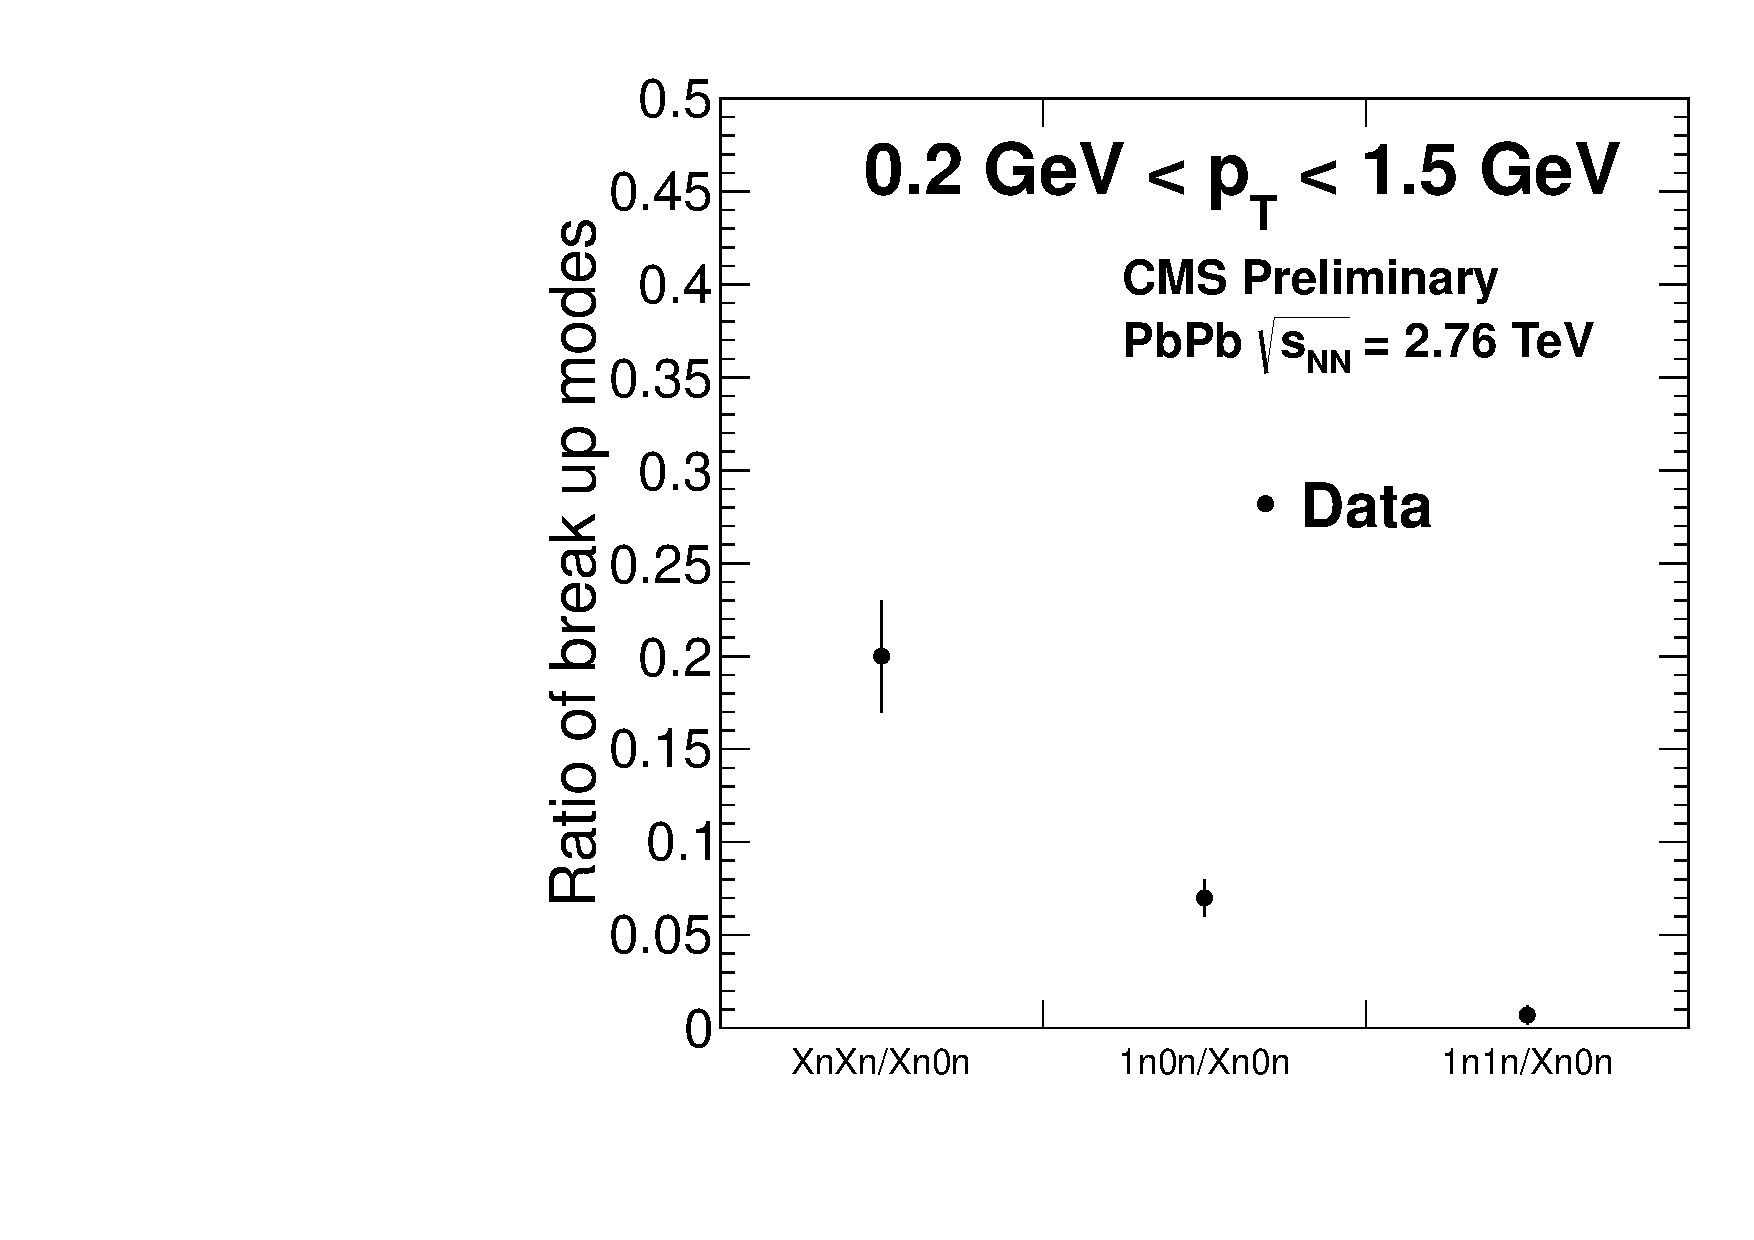
\includegraphics[width=.6\textwidth]{incoherentBreakup}
      \caption{Ratio between J/$\psi$ yeilds XnXn and 1n0n break-up modes 
        compared the Xn0n break-up mode for J/$\psi$ with 0.2 $< p_{T} <$ 
        1.5 GeV.}
      \label{fig:incoherentBreakUp}
    \end{figure}

    The number of the coherent and incoherent J/$\psi$ for each break-up mode are
      given in the Tab.~\ref{tab:r1}. 
    The ratios between the modes X$_{n}$X$_{n}$, 1$_{n}$0$_{n}$, 1$_{n}$1$_{n}$ and
      the mode  X$_{n}$0$_{n}$ are given in the table Tab.~\ref{tab:r2}. 
    Some of the  ratios can be obtained from  {\sc starlight} and from the Zhalov 
      and thus are given in Tab.~\ref{tab:r3}.
    \begin{table}[h]
      \begin{center}
      \begin{tabular}{|c|c|c|c|c|c|}
        \hline
         &  X$_{n}$0$_{n}$& X$_{n}$X$_{n}$ & 1$_{n}$0$_{n}$ & 1$_{n}$1$_{n}$  \\ \hline
        coherent J/$\psi$ &  242$\pm$16&94$\pm$10&58$\pm$8&8$\pm$3\\ \hline
        incoherent J/$\psi$ & 291$\pm$17&57$\pm$8&19$\pm$4&2$\pm$1\\ \hline
      \end{tabular}
      \caption{\label{tab:r1} Number of coherent J/$\psi$ integrated over $p_{T}$ and $y$ 
        with statistical uncertainty.}
      \end{center}
    \end{table}
    
    \begin{table}[h]
      \begin{center}
        \begin{tabular}{|c|c|c|c|c|}
          \hline
          & X$_{n}$X$_{n}$/X$_{n}$0$_{n}$ & 1$_{n}$0$_{n}$/X$_{n}$0$_{n}$ & 1$_{n}$1$_{n}$/X$_{n}$0$_{n}$  \\ \hline
          coherent J/$\psi$ &  0.39$\pm$0.05&0.24$\pm$0.04&0.03$\pm$0.01\\ \hline
          incoherent J/$\psi$ &  0.20$\pm$0.03&0.07$\pm$0.02&0.007$\pm$0.005 \\ \hline
        \end{tabular}
      \caption{\label{tab:r2} Number of coherent J/$\psi$ integrated over $p_{T}$ and $y$ 
        with statistical uncertainty.}
      \end{center}
    \end{table}

    In Table~\ref{tab:r3} the ratio between break up modes are shown for 
      different theories and processes.
    \begin{table}[h]
      \begin{center}
        \begin{tabular}{|c|c|c|c|c|}
          \hline
          & X$_{n}$X$_{n}$/X$_{n}$0$_{n}$ & 1$_{n}$0$_{n}$/X$_{n}$0$_{n}$ & 1$_{n}$1$_{n}$/X$_{n}$0$_{n}$  \\ \hline
          STARlight coherent &  0.37&-&0.02\\ \hline
          Zhalov coherent& 0.32&0.30&0.02\\ \hline
          STARlight incoherent &  0.37&-&0.007$\pm$0.02 \\ \hline
        \end{tabular}
        \caption{\label{tab:r3} Number of  J/$\psi$ integrated over $p_{T}$ and $y$ with 
          statistical uncertainty.}
      \end{center}
    \end{table}
\fi

